\documentclass[a4paper]{article} 
\addtolength{\hoffset}{-2.25cm}
\addtolength{\textwidth}{4.5cm}
\addtolength{\voffset}{-3.25cm}
\addtolength{\textheight}{5cm}
\setlength{\parskip}{0pt}
\setlength{\parindent}{0in}

%----------------------------------------------------------------------------------------
%	PACKAGES AND OTHER DOCUMENT CONFIGURATIONS
%----------------------------------------------------------------------------------------

\usepackage{blindtext} % Package to generate dummy text
\usepackage{charter} % Use the Charter font
\usepackage[utf8]{inputenc} % Use UTF-8 encoding
\usepackage{microtype} % Slightly tweak font spacing for aesthetics
\usepackage[english, ngerman]{babel} % Language hyphenation and typographical rules
\usepackage{amsthm, amsmath, amssymb} % Mathematical typesetting
\usepackage{float} % Improved interface for floating objects
\usepackage[final, colorlinks = true, 
            linkcolor = black, 
            citecolor = black]{hyperref} % For hyperlinks in the PDF
\usepackage{graphicx, multicol} % Enhanced support for graphics
\usepackage{xcolor} % Driver-independent color extensions
\usepackage{marvosym, wasysym} % More symbols
\usepackage{rotating} % Rotation tools
\usepackage{censor} % Facilities for controlling restricted text
\usepackage{listings, style/lstlisting} % Environment for non-formatted code, !uses style file!
\usepackage{pseudocode} % Environment for specifying algorithms in a natural way
\usepackage{style/avm} % Environment for f-structures, !uses style file!
\usepackage{booktabs} % Enhances quality of tables
\usepackage{tikz-qtree} % Easy tree drawing tool
\tikzset{every tree node/.style={align=center,anchor=north},
         level distance=2cm} % Configuration for q-trees
\usepackage{style/btree} % Configuration for b-trees and b+-trees, !uses style file!
\usepackage[backend=biber,style=numeric,
            sorting=nyt]{biblatex} % Complete reimplementation of bibliographic facilities
\addbibresource{ecl.bib}
\usepackage{csquotes} % Context sensitive quotation facilities
\usepackage[yyyymmdd]{datetime} % Uses YEAR-MONTH-DAY format for dates
\renewcommand{\dateseparator}{-} % Sets dateseparator to '-'
\usepackage{fancyhdr} % Headers and footers
\pagestyle{fancy} % All pages have headers and footers
\fancyhead{}\renewcommand{\headrulewidth}{0pt} % Blank out the default header
\fancyfoot[L]{} % Custom footer text
\fancyfoot[C]{} % Custom footer text
\fancyfoot[R]{\thepage} % Custom footer text
\newcommand{\note}[1]{\marginpar{\scriptsize \textcolor{red}{#1}}} % Enables comments in red on margin

%----------------------------------------------------------------------------------------

\begin{document}

%-------------------------------
%	TITLE SECTION
%-------------------------------

\fancyhead[C]{}
\hrule \medskip % Upper rule
\begin{minipage}{0.295\textwidth} 
\raggedright
\footnotesize
\textbf{Jaime Andres Torres Bermejo} \hfill\\   
202014866\hfill\\
j.torres16@uniandes.edu.co

\textbf{Santiago Latorre} \hfill\\  
202111851 \hfill\\  
s.latorre@uniandes.edu.co

\end{minipage}
\begin{minipage}{0.4\textwidth} 
\centering 
\large 
Caso 4\\ 
\normalsize 
Infraestructura Computacional - Universidad de los Andes\\ 
\end{minipage}
\begin{minipage}{0.295\textwidth} 
\raggedleft
\today\hfill\\
\end{minipage}
\medskip\hrule 
\bigskip

%-------------------------------
%	CONTENTS
%-------------------------------
\section{Detalles del Problema.}

\textbf{Nota: gran parte de los detalles son extraidos del entorno de contexto.}

En este caso se estudiarán las necesidades de infraestructura de Finandes, una empresa ficticia que se dedica a la
captación y colocación de recursos financieros.

Aunque desde muchos puntos de vista sería deseable poder definir una infraestructura completamente nueva, que
responda a las necesidades de los diferentes procesos de la organización, es poco práctico hacer “borrón y cuenta
nueva” de la infraestructura actual. Por esta razón se debe plantear una transición gradual, que tomará cierto
tiempo, para ir de la infraestructura actual a la ideal. Teniendo en cuenta esto, en la presentación del caso se
incluyen, tanto las características de las aplicaciones y datos que deben ser soportados, como las de la
infraestructura actual, las cuales condicionan la definición de la nueva infraestructura.

Finandes tiene 900.000 afiliados. Además, la empresa tiene 35 oficinas distribuidas en varios municipios del país.
En todas ellas se prestan los mismos servicios y todas tienen acceso electrónico al centro de datos ubicado en
Bogotá. Se estima que hay unos 50 funcionarios haciendo transacciones de recepción de documentos. Estas
transacciones son dirigidas por un BPM que encadena los procesos de validación de datos e información hasta darle
respuesta a la persona que solicita un trámite.

El servicio que presta la entidad es un servicio de alta sensibilidad social por lo que requiere un nivel de continuidad
alto; los servicios informáticos deben estar disponibles en las oficinas en las horas laborales (de lunes a viernes de
9 am a 3 pm), y vía Internet los siete días de la semana entre 7 a.m. y 12 p.m. Además, se considera que el servicio
al afiliado, el cual es una prioridad en este momento, depende totalmente de un buen funcionamiento de los
sistemas de información, lo cual implica, no sólo que las aplicaciones deben estar disponibles, sino que el tiempo
de respuesta desde cualquier oficina y desde Internet debe ser menor o igual a 3 segundos. Por la razón anterior,
se ha determinado que las aplicaciones de apoyo a la atención al público estén siempre disponibles en el horario
indicado (no se desea que en los sitios de atención se diga que no hay servicio porque no hay línea, como ocurre
eventualmente en la actualidad)

Por las razones mencionadas, se requiere un plan de continuidad para el caso de que haya un incidente mayor que
impida que el centro de datos funcione adecuadamente.

La información más importante que maneja la empresa tiene que ver con los recursos manejados tanto por
personas jurídicas como naturales. En el caso de las empresas, Finandes se ocupa de sus pagos de nómina y las
gestiones financieras propias de una empresa. En el caso de las personas, Finandes ofrece productos de inversión y
préstamos personales.

Los datos son de dos tipos: anteriores y posteriores a la reforma tributaria de este año. En cuanto al primer tipo de
datos, Finandes debe gestionar la información de los recursos manejados por Finandes previo a la mencionada
reforma, junto con las reglas de negocio implementadas para responder a la reglamentación correspondiente. En
lo que concierne a la segunda tipología de datos Finandes debe gestionar la información de los recursos manejados
junto con la reglamentación que los rige. Se va a requerir una nueva base de datos homogénea para los dos tipos
de datos.

Ante las dificultades que ha tenido con su operación, Finandes ha decidido privilegiar la subcontratación de servicios
en la medida de lo posible, lo cual se aplica, entre otros, a aspectos que tengan que ver con las tecnologías de
información y comunicaciones, así como con captura y digitación de datos. Así mismo, está migrando a
transacciones sin papel haciendo que el usuario incremente el número y tipo de transacciones que realiza vía
electrónica (app y web).

La empresa tiene algún retraso tecnológico y se desea transformarla para que cuente con una infraestructura
tecnológica moderna que le permita desempeñar cabalmente sus funciones. Para esto ha decidido renovar su
infraestructura y el objetivo es que esto pueda ser hecho en el menor tiempo posible. Después de un análisis
cuidadoso se ha establecido que esta debe continuar centralizada, con sede en Bogotá.

El proceso de afiliación está subcontratado con una entidad externa y esta reporta periódica y electrónicamente la
información correspondiente, para ser procesada en forma batch. Con base en ella se procede a actualizar las bases
de datos de la entidad.

El proceso de captación lo hacen las sucursales a nivel nacional. El manejo relacionado con préstamos es intenso en
procesamiento pues se requiere hacer conciliaciones tripartitas entre los recursos disponibles, el registro de
transacciones del usuario y las captaciones y colocaciones de la entidad. Estos procesos implican varias verificaciones generan archivos con las inconsistencias encontradas. También se requiere el cobro de intereses no
realizados. Este proceso implica el control del debido pago de los clientes.
Los procesos de analítica encadenan diferentes aplicaciones y bases de datos mediante un flujo de trabajo de estilo
BPM, así como un análisis de las redes sociales de los clientes.

La aplicación de nómina ofrece dos servicios: consultas diarias y consolidación a fin de mes. El primero necesita un
tiempo de respuesta mínimo pues los empleados usan la consulta para atender en las oficinas de servicio al público.
El segundo servicio se realiza a fin de mes, su procesamiento es tipo batch y puede durar varios días. Además, por
su impacto una falla sería muy costosa. Este sistema debe tener un esquema de contingencia totalmente probado
y certificado.

El portal web y la app debe permitir un número creciente de operaciones tanto para personas jurídicas como
naturales.

Se calcula que en la empresa hay aproximadamente 15 bases de datos que ocupan en total 100 terabytes de
espacio. Las bases de datos más importantes, las relacionadas con afiliados y empresas, son usadas por la mayoría
de las aplicaciones. En particular, son usadas por dos aplicaciones, captación y nómina, las cuales deben tener una
alta disponibilidad y un buen tiempo de respuesta. Además, como se dijo arriba, hay que tener mucho cuidado con
las intensivas en procesamiento porque podrían generar problemas de contención.
Las copias de respaldo (“backups”) deben permitir la operación de las aplicaciones misionales durante las horas
hábiles.

La continuidad de la operación está garantizada hoy con la contratación de un centro de datos alterno en otra
ciudad, cuyas bases de datos deben estar sincronizadas con las de la entidad. Esto quiere decir que cualquier
transacción que se haga en la entidad se debe reflejar también en el centro alterno. Este centro de datos es
administrado por la entidad encargada de hacer las afiliaciones.
Todas las sucursales tienen conexión al centro de datos central, el cual reside en Bogotá. De ellas, 12 están ubicadas
en la ciudad de Bogotá. Se desea que el procesamiento se siga haciendo de forma centralizada, en Bogotá.
Además de lo anterior, la entidad debe conectarse electrónicamente con 5 puntos ubicados en entidades externas
(por ejemplo, la empresa que se encarga de las afiliaciones, el banco de la república y la superfinaciera). Hay una
conexión especialmente importante que es la actualización en línea con el centro de datos alterno, el cual está
ubicado en otra ciudad.

Hace aproximadamente un año, el servidor activo fue repotenciado, aumentando su capacidad de memoria y
procesamiento (10 procesadores físicos Xeon EPY C 73F3 y 128GB de memoria RAM). El proveedor del manejador
de base de datos Oracle, ha sugerido que la configuración mínima de memoria RAM de este servidor sea de 512 GB
(la máxima posible en ese servidor). Cada nuevo slot de 64GB cuesta aproximadamente 100 millones de pesos. Este
servidor también puede ser actualizado con procesadores con más núcleos, con un costo aproximado de 10 millones
de pesos por procesador. El costo anual de licenciamiento de Oracle por núcleo de procesador es de
aproximadamente 10 millones de pesos.

El servidor pasivo es menos poderoso que el activo y se estima que en caso de falla es poco probable que pueda
asumir toda la carga del sistema

\subsection{Principios tecnológicos}

Dentro de los principios tecnológicos que se han definido en la empresa con respecto a la infraestructura están los
siguientes: el procesamiento debe ser centralizado, se continuará con la subcontratación de las afiliaciones y el
centro alterno, se seguirá trabajando con procedimientos almacenados, se trabajará con el ambiente de desarrollo
de Java y con el ambiente de bases de datos Oracle. Puede que algunas de estos principios cambien en el mediano,
pero no en el corto plazo.

Existen también otros lineamientos:
\begin{itemize}
    \item Exigir que los terceros contratados dispongan de planes de contingencia y continuidad debidamente
    documentados.
    \item Implementar mecanismos de cifrado fuerte para el envío y recepción de información confidencial con los
    terceros contratados.
\end{itemize}

\subsection{Infraestructura existente}
Dado el enunciado dado arriba, sabemos que tenemos, bajo control completo de la compañía:
\begin{itemize}
    \item un BPM (Business Process Manager)
    \item un portal web (sin especificaciones de frameworks o tecnologías)
    \item una app movil (sin especificaciones de frameworks o tecnologías)
    \item 37 servidores (solo nos centraremos en aquellos afectados por la estructura TO-BE)
    \item 15 bases de datos con 100 TB de datos.
    \item conexiones con el banco, la superfinanciera, y las aplicaciones para las aplicaciones.
\end{itemize}

Y, tenemos de forma subcontratada:

\begin{itemize}
    \item Un proceso de subcontratación.
    \item los servicios de conexión tienen software propietario que no controlamos como parte de su servicio. 
    se asumirá como una caja negra este producto dentro de nuestro diseño.
    \item un centro de datos alterno. 
\end{itemize}

Fuera de esto, se va a asumir que:

\begin{itemize}
    \item La arquitectura de las aplicaciones, basada en procedimientos almacenados (“stored procedures”), dificulta la
    distribución de la carga computacional requerida para su funcionamiento lo que contribuye a los problemas de
    sobrecarga de los servidores de base de datos institucionales.
    \item La mayoría de los servidores tienen más de 4 años de uso (algunos tienen más de 10 años de uso). Hay
    aproximadamente 39 servidores físicos en el centro de cómputo.
    \item En lo que se refiere a los servidores de apoyo a las bases de datos, que son actualmente dos, organizados en
    un clúster activo-pasivo, se ha determinado que están sobrecargados.
\end{itemize}

Estas reglas se pueden visualizar a partir del siguiente diagrama:
\begin{center}
    \textbf{Modelo de aplicaciones AS-IS}
    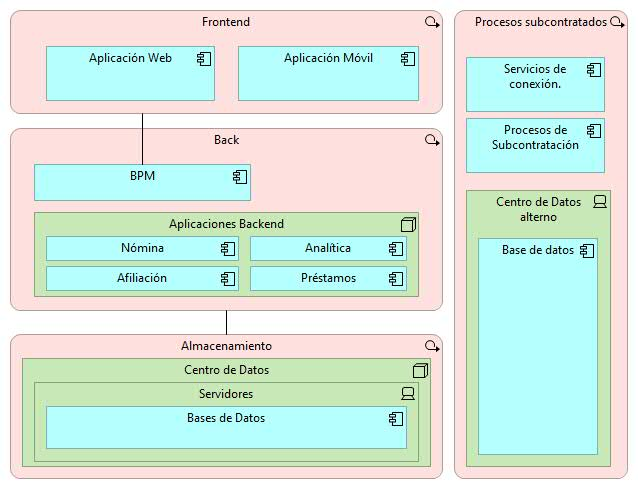
\includegraphics[scale=0.56]{as-is.jpg}    
\end{center}

\section{Diseño de las soluciones.}

\subsection{secciones a evaluar.}
Hay 7 principales secciones que se evaluarán:
\begin{itemize}
    \item Afiliación: 100 transacciones al día que se procesan en la noche y que generan mucha carga de
    entrada/salida en almacenamiento
    \item Captación: estos ingresos de dinero, de los cuales hay unos 20,000 al día, se consolidan en la noche y
    generan mucha carga en almacenamiento.
    \item Préstamos: 4,000 operaciones diarias que se deben resolver en línea y que requieren alta capacidad de
    cómputo
    \item Analítica: se ejecutan unas 500 diarias, la mitad de las cuales son en línea y son grandes consumidoras de
    procesamiento.
    \item Nómina: Se procesan unas 20,000 a finales de mes con alto consumo de procesamiento y de operaciones
    de entrada/salida
    \item App y Web: se espera pasar de 2.000 a 10,000 operaciones diarias en los próximos meses. Son intensivas
    en operaciones de entrada/salida
\end{itemize}

Para cada una de estas, se desarrollará una arquitectura diferente teniendo en cuenta sus requerimientos.
Los requerimientos se van a clasificar como:
\begin{itemize}
    \item \textbf{Desempeño}
    \item \textbf{Disponibilidad}
    \item \textbf{Escalabilidad}
    \item \textbf{Capacidad}
\end{itemize}

Para estos casos de uso, se establecen los siguientes requerimientos:

\textbf{General:}
\begin{itemize}
    \item En general todo se espera poder mantener en una misma granja de servidores, sin el uso de multinube.
    \item Debe poder reutilizarse la tecnología existente, dado a que esto reduce costos
\end{itemize} 

\textbf{Afiliación:}
\begin{itemize}
    \item \textbf{Desempeño}
    
    La carga de entrada/salida es muy intensiva, por lo que la solución debe poder 
    hacer estas operaciones de forma satisfactoria.
    
    \item \textbf{Disponibilidad}
    
    Dado que la aplicación se usa de forma diaria, debe estar disponible de forma relativamente
    constante.

    \item \textbf{Escalabilidad}
    
    La carga es procesada en la noche, por lo que es perfectamente posible escalar
    y desescalar en medida de que sea necesario. 

\end{itemize}

\textbf{Captación:}
\begin{itemize}
    \item \textbf{Escalabilidad}
    
    Dado que este servicio solamente se utiliza a finales de mes, solamente es necesario mantener
    este servicio durante ese espacio de tiempo, por lo que debe poder escalarse la capacidad del 
    servicio para acomodar la demanda, pero pueden quitarse dichos recursos en las ocasiones que 
    no sean utilizados.

    \item \textbf{Capacidad}
    
    Esta es la aplicación que tiene el mayor número de peticiones en un periodo corto de
    tiempo. Por lo tanto debe poderse procesar de forma eficiente esta cantidad de transacciones
    al final de cada mes sin sobrepasar la barrera de sobrecarga.

\end{itemize}

\textbf{Analítica:}
\begin{itemize}
    \item \textbf{Desempeño}

    Finandes nos ha suministrado una copia de la consulta principal que resuelve la aplicación de Analítica y
    espera su ayuda para determinar la infraestructura de TI necesaria para cumplir con un tiempo de respuesta de
    este servicio menor o igual a 4 segundos por lo menos en el 95 \% de las veces
    
    Gran parte del trabajo hecho de parte de Analítica sera dado con respecto a esta. 
\end{itemize}

\textbf{Nómina:}
\begin{itemize}
    \item \textbf{Desempeño}
    
    La alta necesidad de operaciones de entrada y salida implican una necesidad de que las operaciones sean eficientes.  

    \item \textbf{Capacidad}
    
    Se procesan 20.000 solicitudes en hora pico. Es la aplicación que requiere una mayor capacidad 
    al ser utilizada.

\end{itemize}

\textbf{App y Web:}
\begin{itemize}
    \item \textbf{Desempeño}
    
    Gran parte del desempeño de esta aplicación esta fuera de nuestro control, cosas como la conexión del
    cliente o la calidad de su conexión puede afectar el servicio. Sin embargo, debe poderse mantener un tiempo
    de respuesta aceptable.

    \item \textbf{Disponibilidad}
    
    Dado que esta es nuestra principal conexión digital con los clientes, es importante que el programa
    tenga una alta disponibilidad. los tiempos de respuesta deben minimizarse u ocultarse al individuo que 
    use la aplicación

    \item \textbf{Escalabilidad} 
    
    Se espera lograr que la aplicación escale su capacidad de 
    2,000 a 10,000 solicitudes por día en los próximos meses. Esto
    implica un aumento permanente de la capacidad del sistema con respecto al
    modelo AS-IS.
    
    \item \textbf{Capacidad}
    
    La capacidad de esta capacidad, aunque no es constante en práctica, se asumirá de forma
    constante. Sin embargo, se asumirá para las pruebas la capacidad máxima

\end{itemize}

\subsection{Diseños individuales}

\subsection{Afiliación}
Debido a que ya se contrato a un tercero que realiza todo el proceso de afiliación, y cuyo objetivo es enviar la información relacionada con este proceso, lo único que queda por evaluar es el procedimiento de recepción de información y guardado en base de datos. Teniendo en cuenta esto, se propone como solución una arquitectura monolítica que reciba la información, y la transforme de manera que se pueda almacenar en la base de datos sin que haya incompatibilidad en formatos o estructuras. Los principales beneficios de esta arquitectura es que, si la máquina tiene buenas especificaciones, el rendimiento de toda la API será optimo, además de que quita lugar a cualquier inconsistencia en la base de datos que podría ocurrir si hay múltiples servicios escribiendo en la base de datos de forma simultánea. Para garantizar que se cumpla el requerimiento de desempeño, se propone un escalamiento vertical del servidor utilizado para esta aplicación, pues aunque puede llegar a ser muy costoso, se trata de uno solo, que además solo necesita estar encendido en las noches, pues es en este tiempo en el que se realiza el proceso.

PD: Dado que esta aplicación procesa la información de forma batch, no hace falta una aplicación web que despliegue el servicio.
\begin{center}
    \textbf{Infraestructura de Afiliación}

    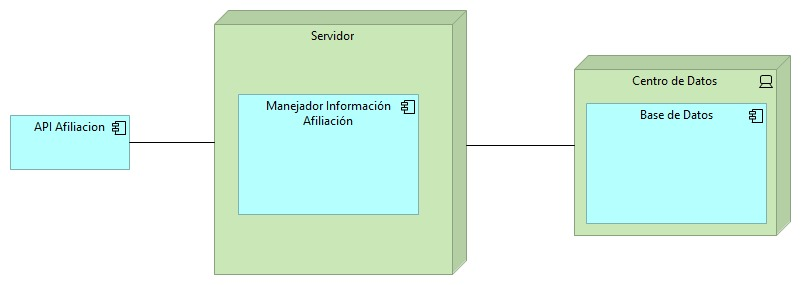
\includegraphics[scale=0.5]{afiliacion.jpeg}
\end{center}

\subsubsection{Préstamos}

Dado el hecho de que este es un servicio demandante en capacidad de cómputo, utilizaremos el 
Servidor activo proveído, previamente repotenciado en la infraestructura existente con el fin de poder 
procesar de forma eficiente las 4000 solicitudes. Vamos a tener al servidor pasivo conectado a este centro
con el fin de procesar casos en el caso de una sobrecarga, que en general debería ser infrecuente para la mayoría
de los casos pero sigue siendo una posibilidad en casos donde este servicio de procesamiento sea consumido por otras
API. También dado a que no se da una hora especifica de uso, es muy posible que la carga este distribuida a lo largo
del día, por lo que será generalmente raro tener 4000 solicitudes ocurriendo a la vez. Esta tomará de Input 
información dada por HTTPS u otra red que nos de la información a ser procesada. Todas estas peticiones serán, de la misma
forma que se puede ver como un tema común en las soluciones propuestas, tomado a partir de una API y  Transmitido a partir de un
Broker al centro de procesamiento, donde dependiendo de la carga actual entrará al servidor activo o pasivo, el cual ayudará
para evitar que se genere un crecimiento exponencial en el tiempo de respuesta. Todos los output irán inmediatamente a la base de datos
de Finandes. En caso de una falla general del servidor activo se pasa la carga al servidor pasivo, esta no es una situación ideal 
para el sistema, e implicaría las operaciones funcionando con un rendimiento limitado. Se espera evitar este escenario 
lo más posible.

\begin{center}
    \textbf{Infraestructura de Préstamos}
    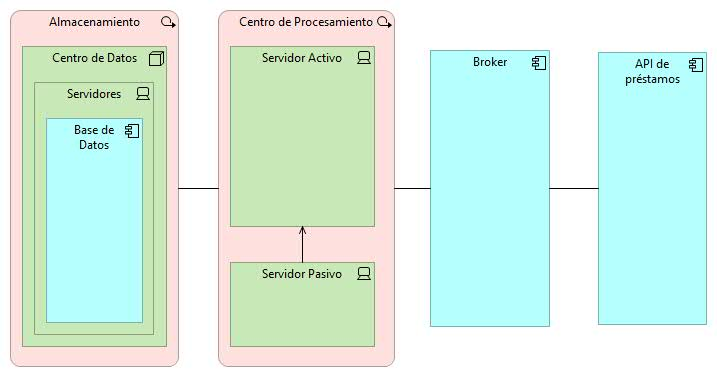
\includegraphics[scale=0.6]{prestamos.jpg}
\end{center}

\subsubsection{Analítica:}

Al observar los resultados obtenidos en las pruebas realizadas a la infraestructura actual, se puede afirmar que esta es sumamente desfavorable para alcanzar los objetivos propuestos, pues como se puede evidenciar en la gráfica, la fórmula que más se ajusta a la recta es y = 13,222x, lo que en otras palabras significa que por cada petición que se envíe a la aplicación, el tiempo de respuesta aumentará 13 segundos aproximadamente. Esto significa que ni siquiera con un único thread se alcanza el límite esperado de 4 segundos, y es un indicador claro de que la infraestructura está sumamente desactualizada, de manera que es de vital importancia realizar mejoras para garantizar que la aplicación cumpla con las necesidades actuales del negocio.
Para determinar el tiempo que la máquina se tarda en manejar 2000 peticiones, podemos utilizar la fórmula de la regresión lineal, obteniendo como resultado
\begin{center}
    y=13,222(2000)=26,644 segundos=7,4 horas    
\end{center}

Siendo este un resultado completamente inaceptable para las tecnologías de la actualidad.
Ahora, si se quiere calcular la cantidad de máquinas necesarias para que el tiempo sea de 4 segundos en total, se puede utilizar la siguiente formula:

\begin{center}
    4= 26,644/(cant maquinas)
    
    cant maquinas= 26,644/4 = 6661 maquinas        
\end{center}

Esto quiere decir que, si se tuviera que utilizar la infraestructura actual para manejar 2000 peticiones en menos de 4 segundos, resultaría necesario contar con mas del triple de consultas, siendo este otro indicador claro de que la arquitectura propuesta no cuenta con la capacidad necesaria para manejar esta cantidad de peticiones, y resulta necesario recurrir a tácticas o estrategias más recientes que permitan abordar esta necesidad. Como sugerencia principal, se recomienda fuertemente recurrir a un escalamiento vertical, porque las máquinas probadas tienen dificultades para procesar incluso una única petición, problema que se puede solucionar aumentando la capacidad de procesamiento y memoria RAM individual. No es recomendable recurrir a otras estrategias como failovers y balanceadores de carga porque, como se evidenció anteriormente, la cantidad de máquinas que sería necesario mantener para poder procesar volúmenes de información importantes es inviable.


\begin{center}
    \textbf{Regresión Lineal de número de threads vs tiempo}
    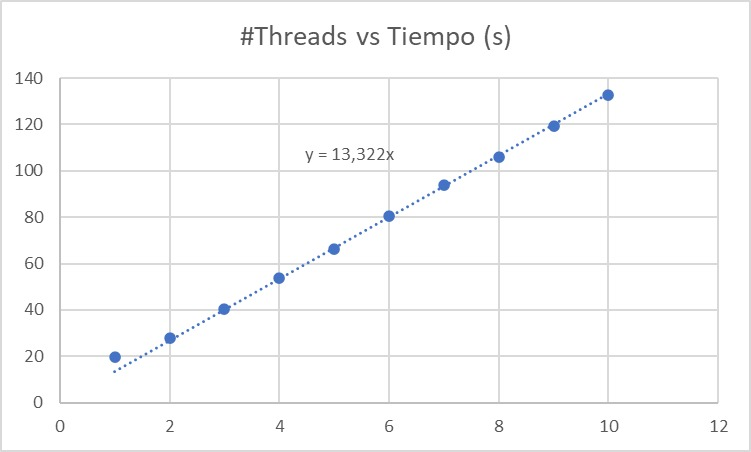
\includegraphics[scale=0.5]{reg_lineal.jpeg}

    \textbf{Tabla de número de threads vs tiempo.}

    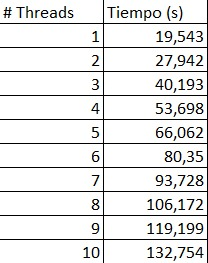
\includegraphics[scale=0.7]{tabla.jpeg}
\end{center}
\subsubsection{Captación}

Teniendo en cuenta la cantidad de funcionalidades y la cantidad de peticiones que llega a recibir esta aplicación, se decidió recurrir a una arquitectura de microservicios, donde cada uno de ellos cuente con varios servidores para garantizar todos los requerimientos identificados. Para enviar las peticiones al microservicio correspondiente se hace uso de una API GATEWAY, que direcciona a la API adecuada (pese a que existe un costo de desempeño al realizar el redireccionamiento, para efectos de este caso resulta insignificante). El primer microservicio hace referencia a el manejo de los recursos disponibles, el segundo al registro de transacciones y el tercero al manejo de las captaciones y colocaciones de la entidad. De esta forma cada microservicio trabaja de forma independiente entre sí, y se puede realizar la conciliación entre las tres partes de forma mucho más efectiva, pues errores de un microservicio no afectan a otro, y eficiente, pues los 3 microservicios son independientes entre sí, por lo que pueden trabajar de forma paralela sin ningún tipo de inconveniente. Así mismo, cada microservicio cuenta con su respectiva base de datos, de forma que se distribuya la información según se necesita y se garantiza mayor disponibilidad de las BD al haber menos consultas sobre una sola. 
\begin{center}
    \textbf{Infraestructura de Captación}
    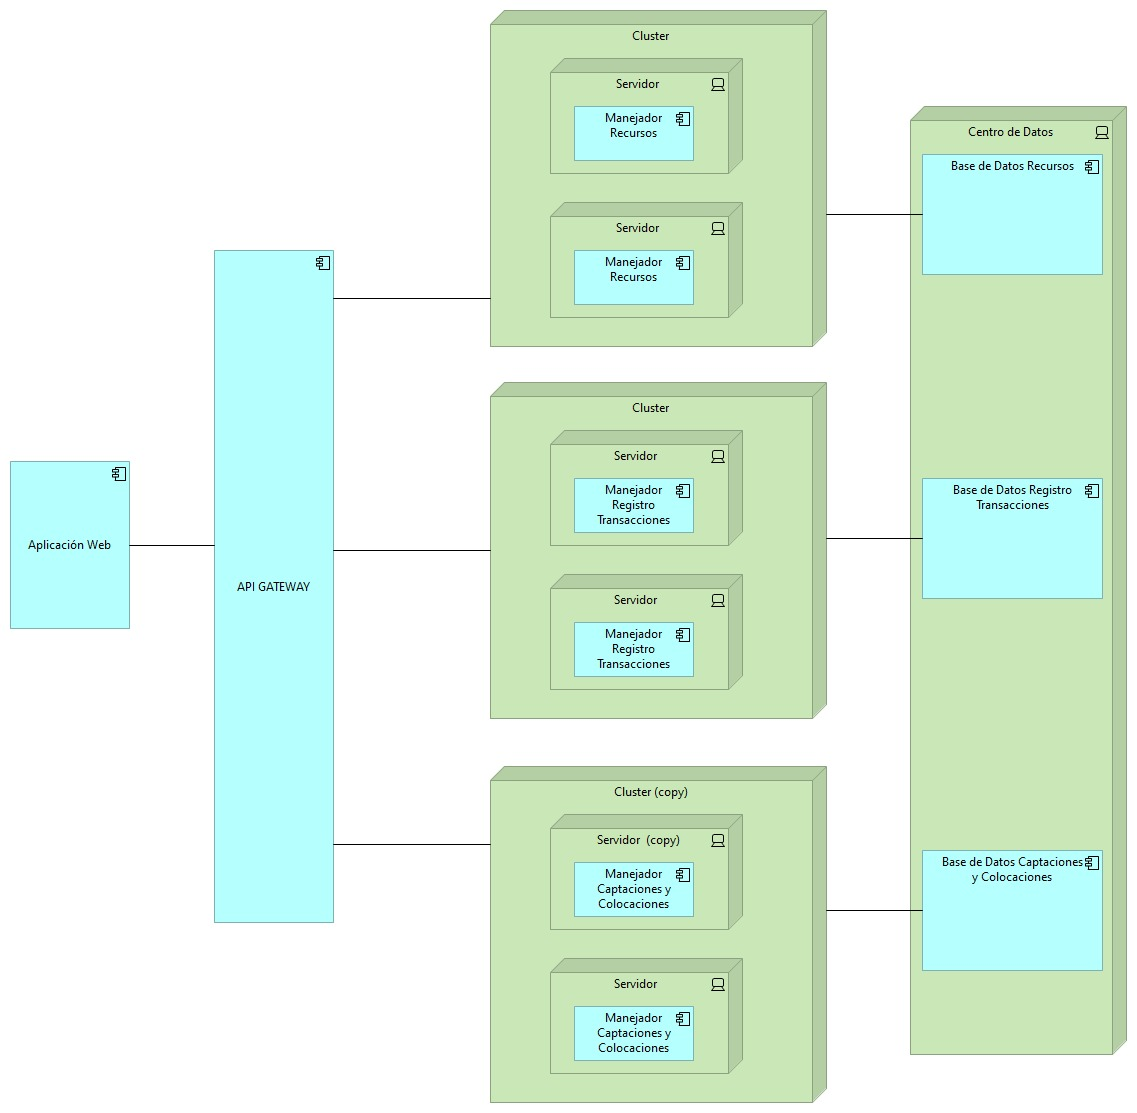
\includegraphics[scale=0.45]{captacion.jpeg}        
\end{center}

\subsubsection{Nómina:}
Teniendo en cuenta que los principales requerimientos que esta sección busca cumplir son desempeño, escalabilidad y disponibilidad, se propone como táctica el uso de un balanceador de carga. De esta forma, las peticiones que lleguen a la aplicación de nómina podrán ser distribuidas entre los servidores activos, garantizando así un mejor desempeño y tiempo de respuesta por parte de la aplicación, además de garantizar que una falla no tenga repercusiones muy importantes en los tiempos y costos. Por otro lado, para garantizar que este escalamiento horizontal no resulte en costos desproporcionados que opaquen los beneficios de la solución, se propone utilizar el mecanismo de redundancia pasiva, de forma que los servidores adicionales no consuman energía mientras no sea necesario, y solo se activen cuando reciban el mensaje de que los servidores se encuentran sobrecargados. 

Un beneficio adicional que ofrece esta táctica es la facilidad para agregar o eliminar servidores de la infraestructura. En otras palabras, si se ve durante las pruebas que no se está aprovechando los recursos adecuadamente, basta con desconectar la maquina del balanceador y reasignarle tareas que resulten de mayor consumo; así mismo, si queda en evidencia que se requieren más procesamiento para cumplir con los tiempos de respuesta definidos, es suficiente conectar una nueva máquina y replicar el contenido de las otras sobre ella, ya que todas cuentan con la misma información.
\begin{center}
    \textbf{Infraestructura de Nómina}
    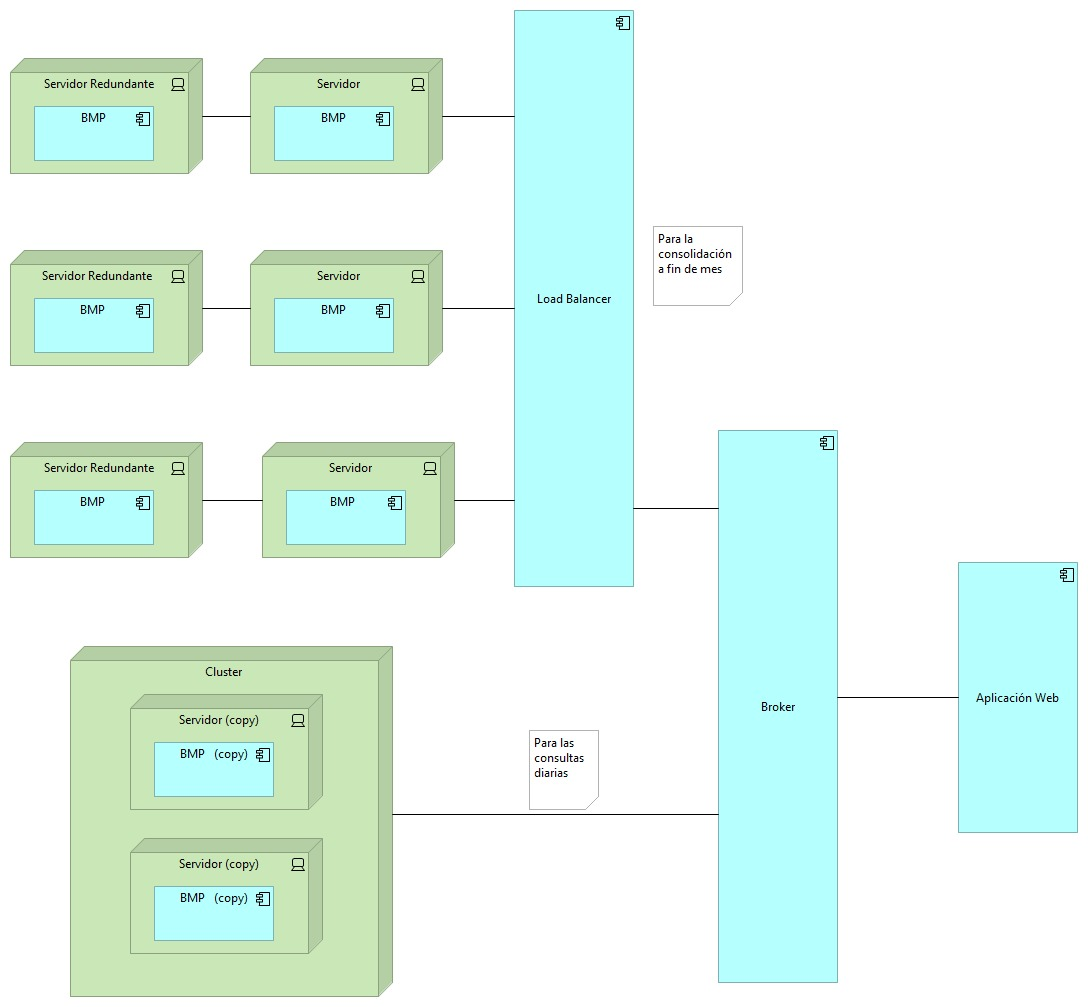
\includegraphics[scale=0.45]{nomina.jpeg}
\end{center}

\subsubsection{App y Web:}

En este diseño, nos va a concerner no necesariamente el diseño interno de las apps de Finandes,
sino su conexión con el resto de la infraestructura. Esto debido a que el diseño web y de las apps
puede cambiar drasticamente entre sí (Swift no es lo mismo que Java, y Java no es lo mismo que Typescript.)
y no le concierne a los temas de este curso. Lo que si nos concierne, sin embargo, es la conexión con el resto
de la infraestructura.

Vamos a entender la infraestructura bajo estas pretensiones:
\begin{itemize}
    \item podemos usar los servidores dentro de la infraestructura AS-IS
    \item Se va a usar un failover dada la necesidad de disponibilidad para este servicio.
    \item Aunque la encriptación hace las transacciones mas lentas, es un mal necesario dada la necesidad por seguridad dentro del negocio.
\end{itemize}

Se va a pensar entonces, dadas estas condiciones, de esta forma la infraestructura:

\begin{center}
    \textbf{Infraestructura de App y Web}
    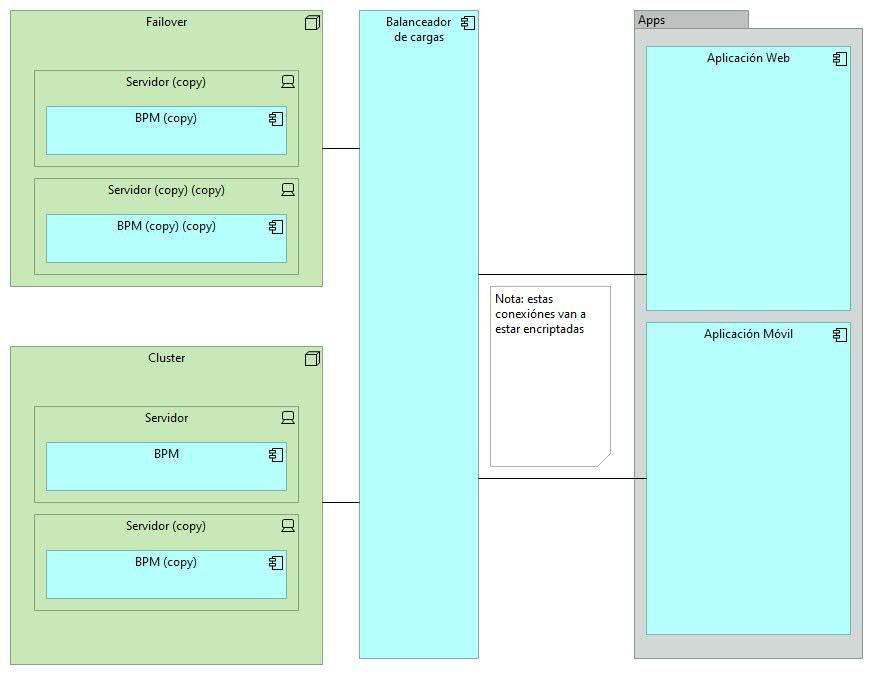
\includegraphics[scale=0.56]{webapp-diagram.jpg}    
\end{center}

%------------------------------------------------
\end{document}
